\documentclass{article}

\usepackage{graphicx}
\usepackage{float}
\usepackage{amssymb}

\title{Machine Intelligence 2 - Exercise 11\\
Stochastic Optimization}
\author{Jens Krenzin - 319308\\
Till Rohrmann - 343756}
\date{\today}

\begin{document}
	\maketitle
	\setcounter{section}{11}
	\setcounter{subsection}{1}
	\subsection{Self-Organizing Maps}
		Initial learning rate $\eta=1$, reduction factor $\eta_{red}=0.99$. Initial sigma $\sigma=\log_{2}(K)$, reduction factor $\sigma_{red}=0.99$.
		\begin{figure}[H]
			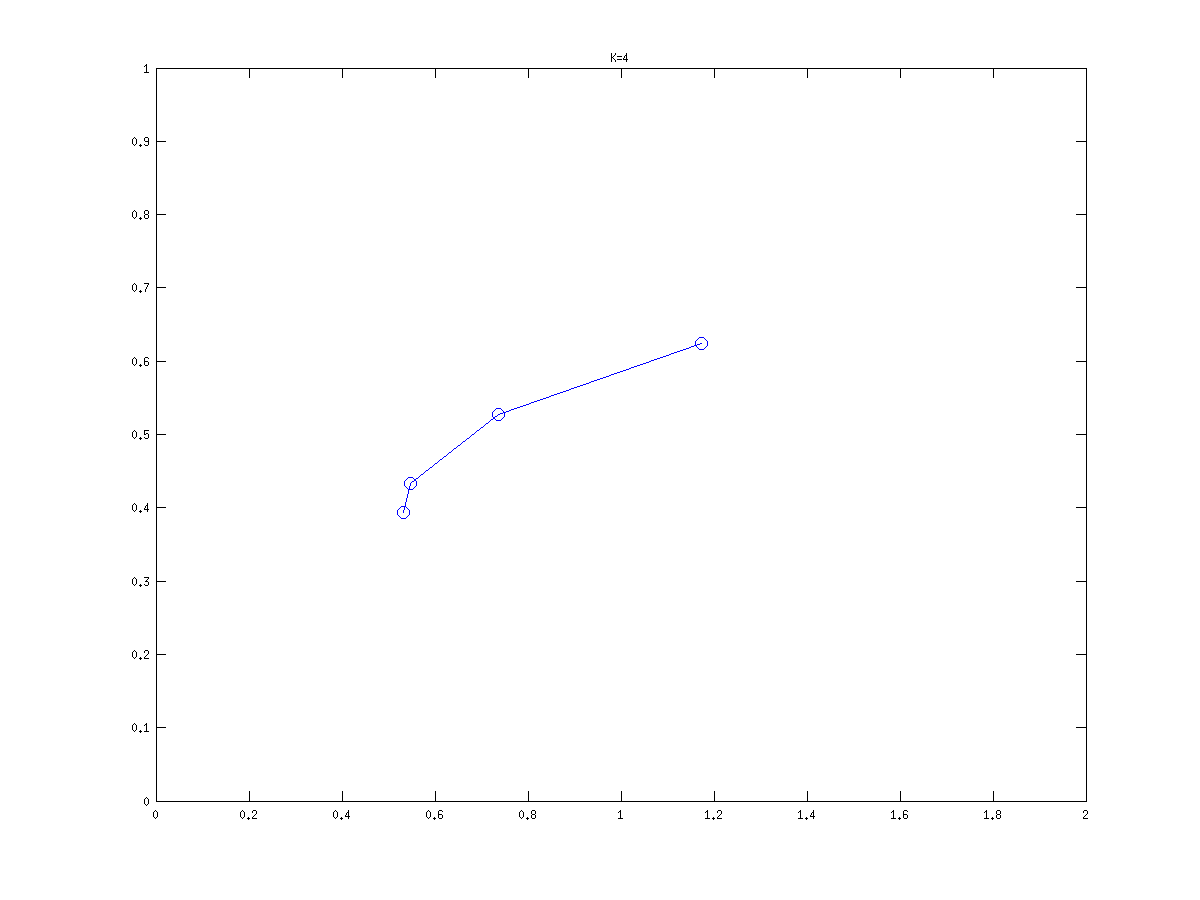
\includegraphics[width=10cm]{k4.png}
			\caption{K=4}
		\end{figure}
		\begin{figure}[H]
			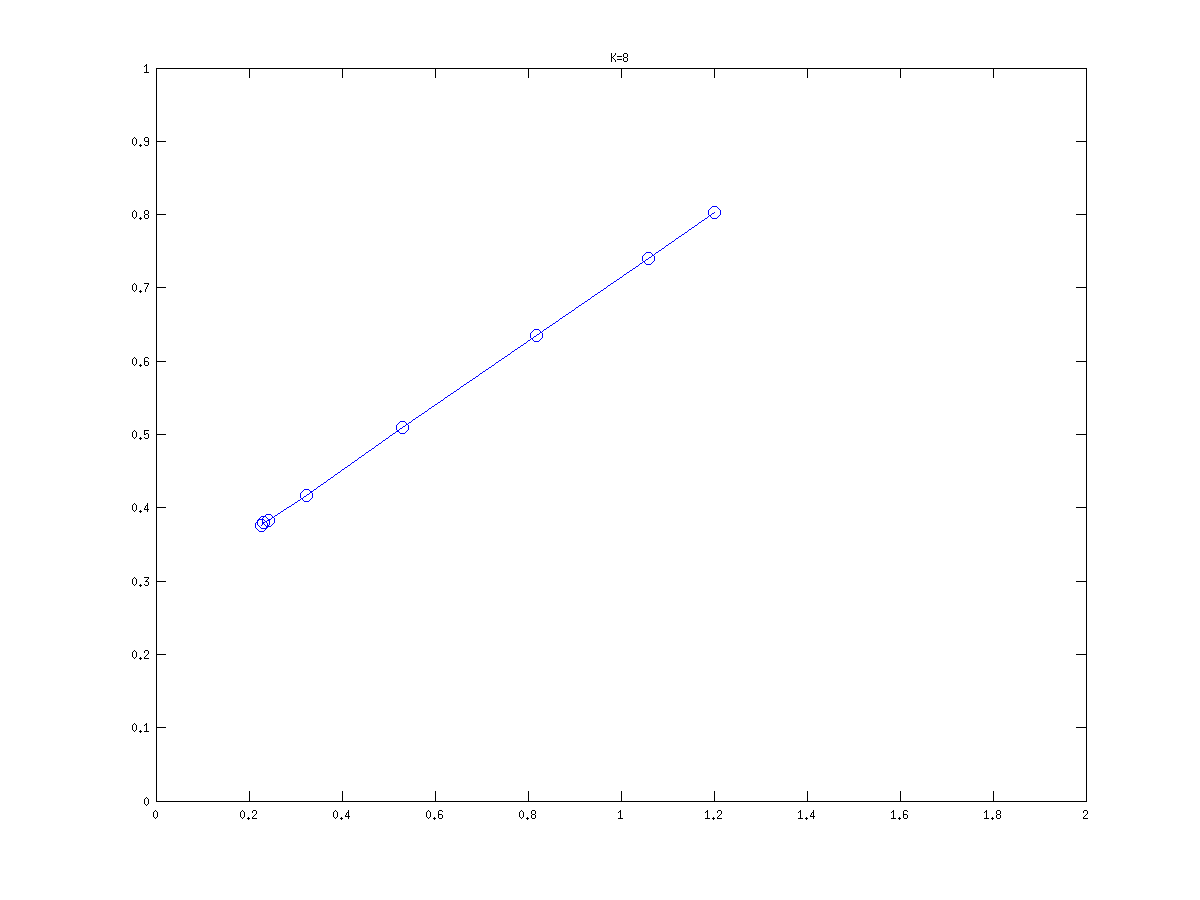
\includegraphics[width=10cm]{k8.png}
			\caption{K=8}
		\end{figure}
		\begin{figure}[H]
			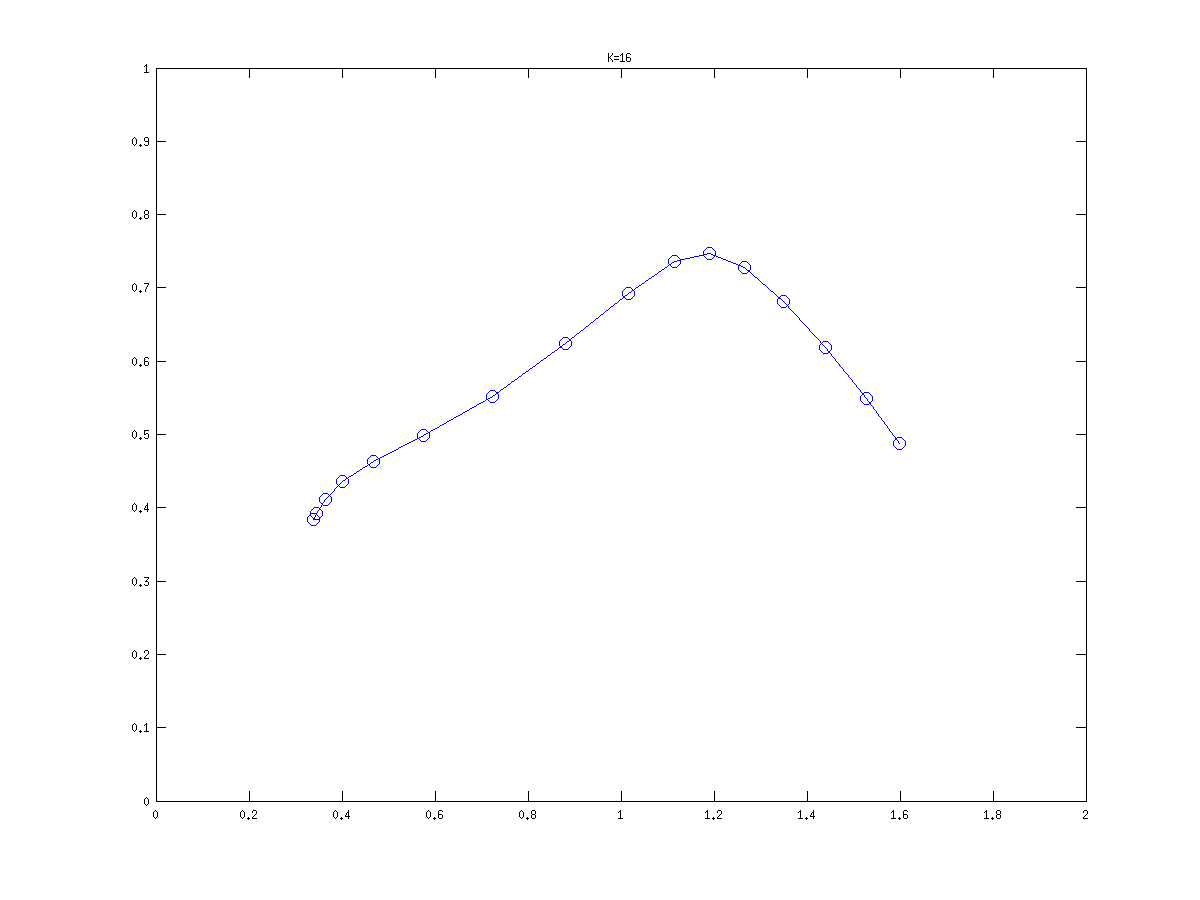
\includegraphics[width=10cm]{k16.png}
			\caption{K=16}
		\end{figure}
		\begin{figure}[H]
			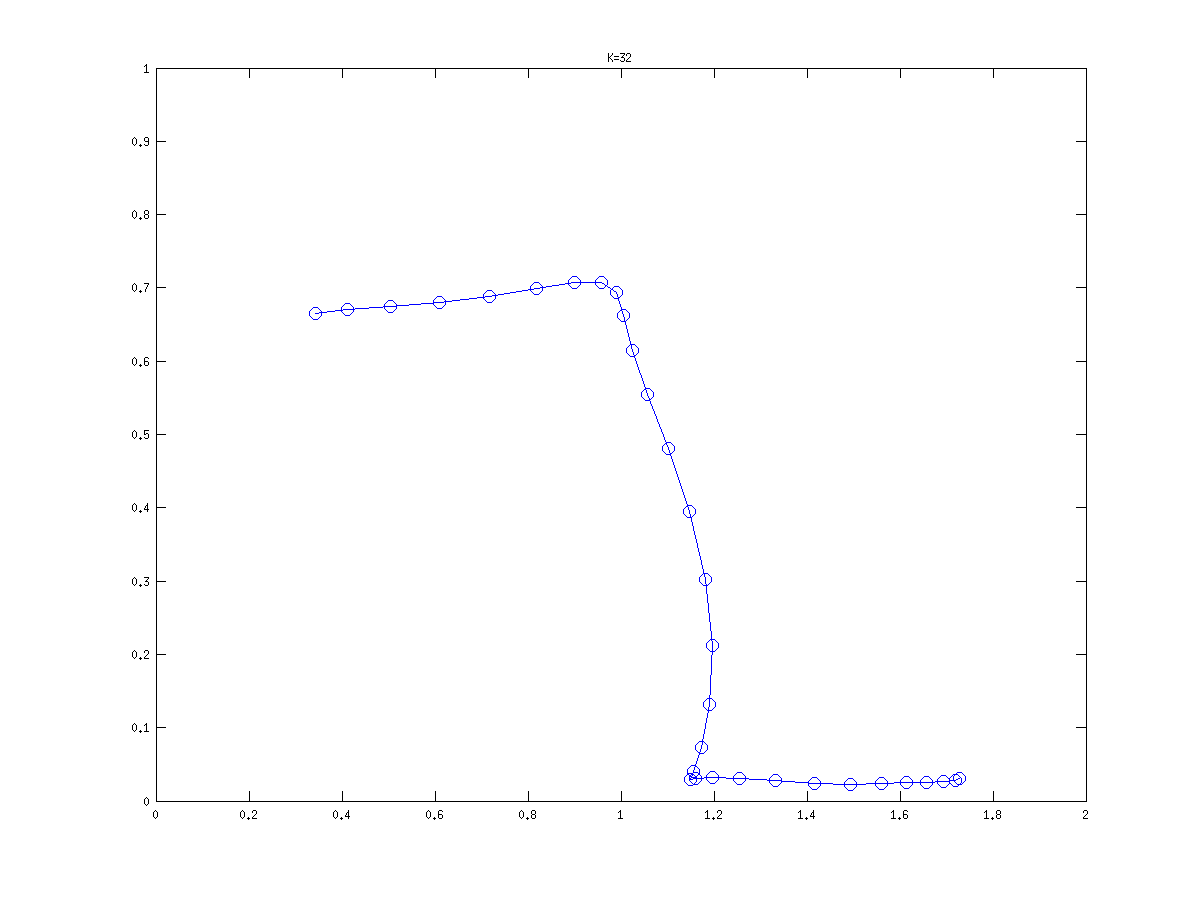
\includegraphics[width=10cm]{k32.png}
			\caption{K=32}
		\end{figure}
		\begin{figure}[H]
			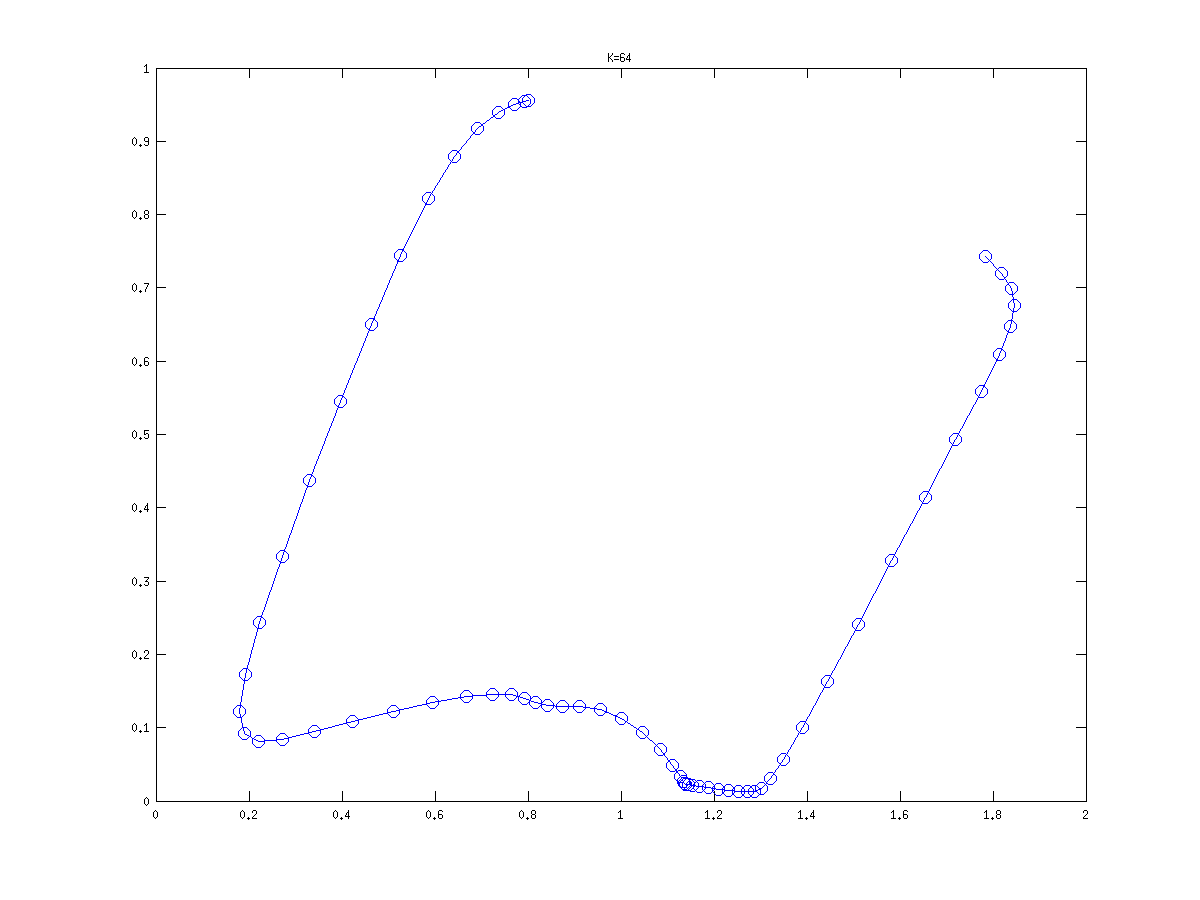
\includegraphics[width=10cm]{k64.png}
			\caption{K=64}
		\end{figure}
	\subsection{Mean-Field Annealing}
		
		\begin{figure}[H]
			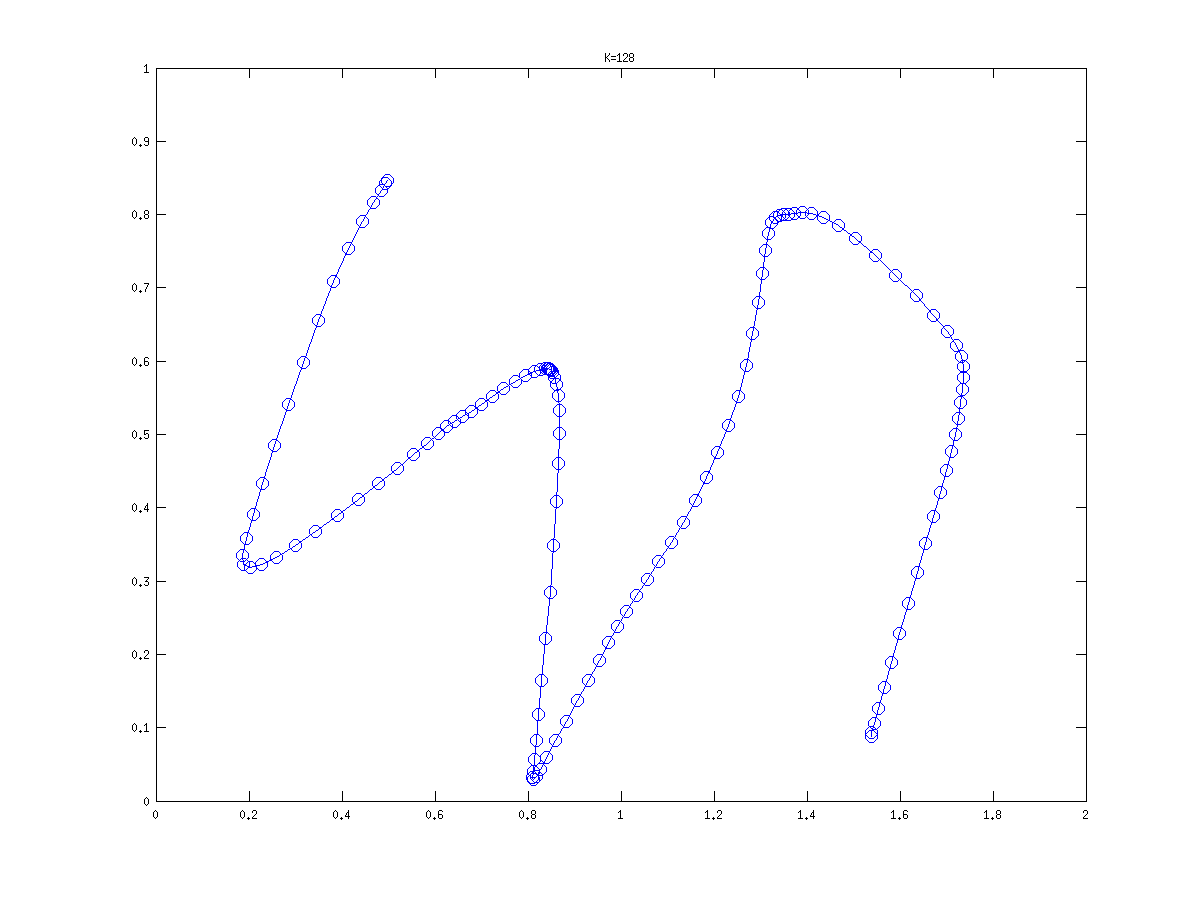
\includegraphics[width=10cm]{k128.png}
			\caption{K=128}		
		\end{figure}	
		
		\begin{figure}[H]
			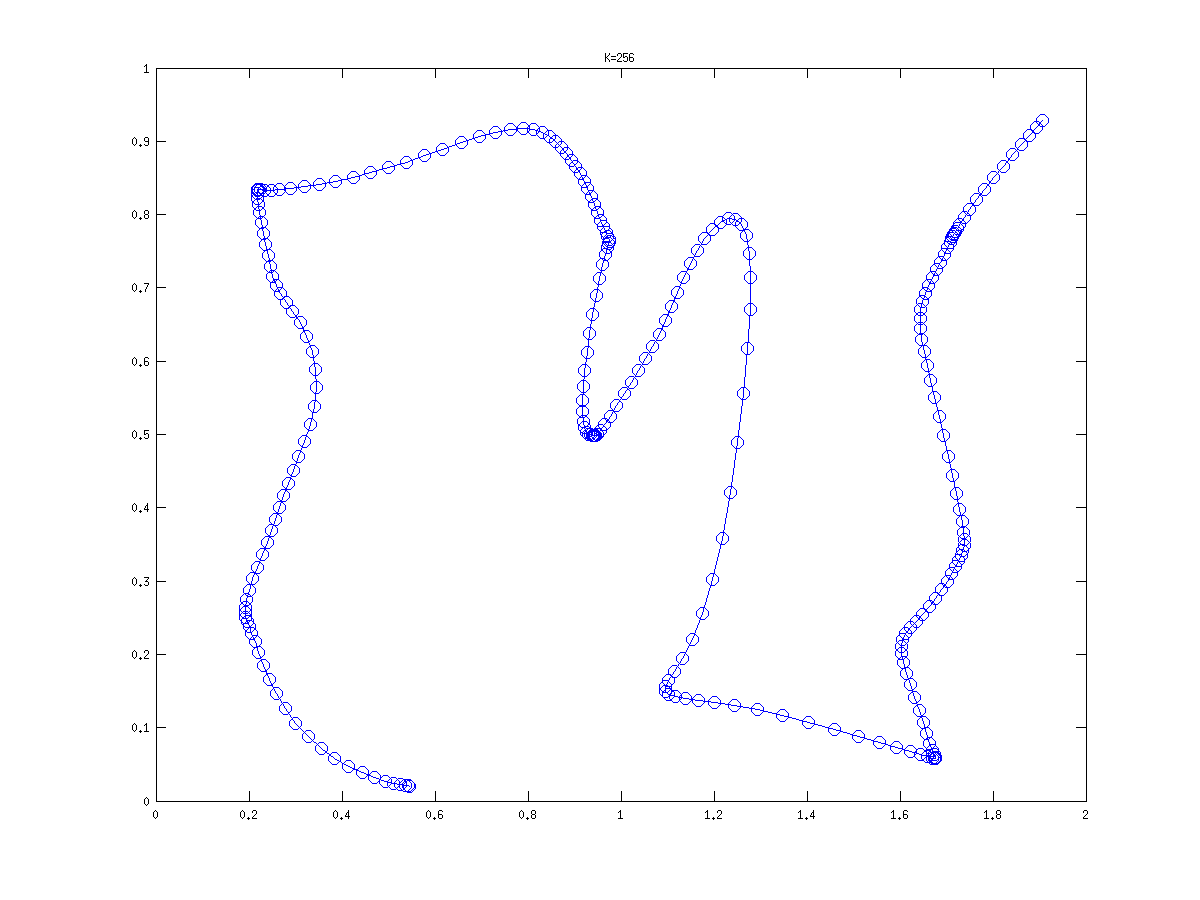
\includegraphics[width=10cm]{k256.png}
			\caption{K=256}
		\end{figure}
		
		\begin{figure}[H]
			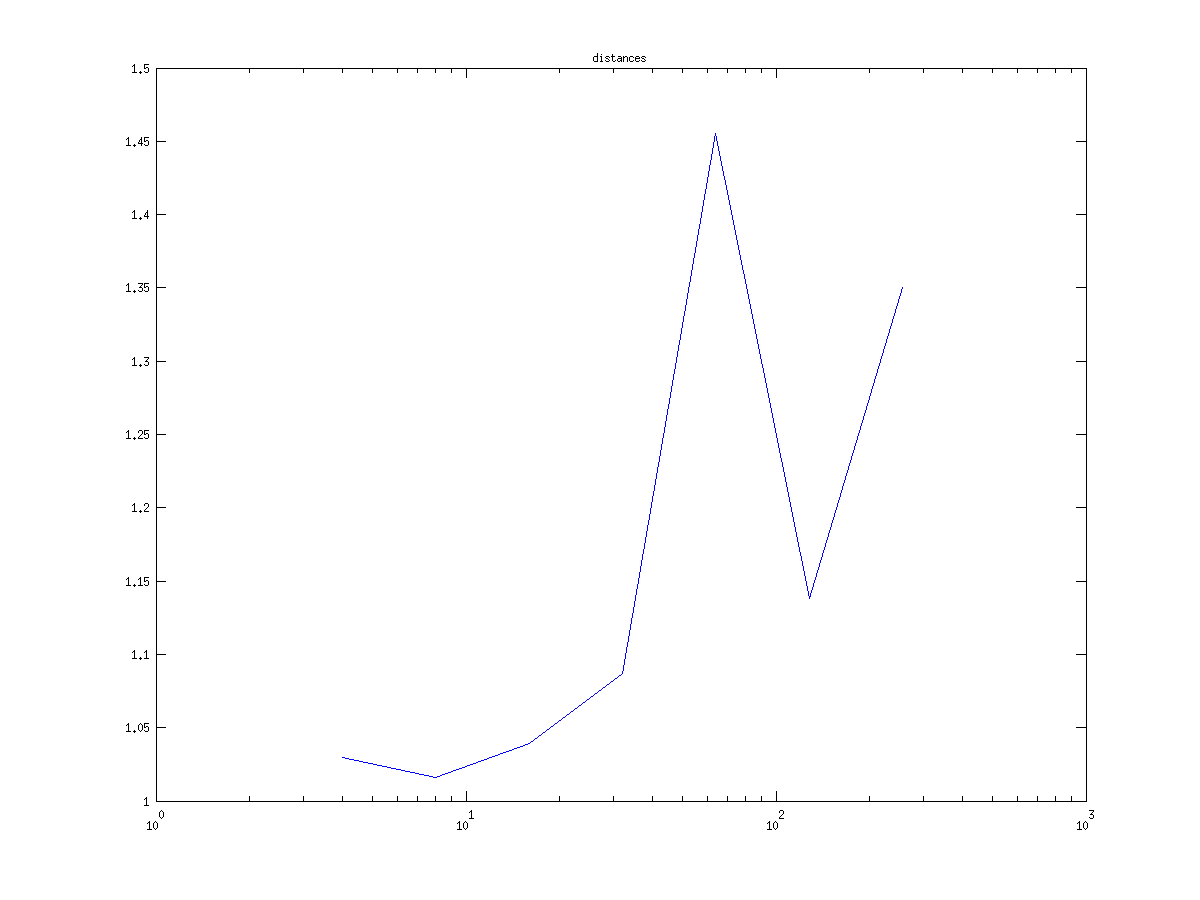
\includegraphics[width=10cm]{distances.png}
			\caption{Average distances between the best and the second best fit measured in map space distance.}
		\end{figure}
	
\end{document}
